\documentclass[final]{beamer}


% ====================
% Packages
% ====================

\usepackage[T1]{fontenc}
\usepackage{lmodern}
\usepackage[orientation=portrait,size=a2,scale=1.15]{beamerposter}
\usepackage{ragged2e}

% Estilo de poster autocontenido; compatible con pdfLaTeX.
\usefonttheme{professionalfonts}
\definecolor{azulposter}{RGB}{59,80,99}
\definecolor{grisposter}{RGB}{73,91,106}
\definecolor{rosaposter}{RGB}{255,246,243}
\definecolor{lineaposter}{RGB}{78,80,83}
\setbeamercolor{background canvas}{bg=white}
\setbeamercolor{normal text}{fg=black,bg=white}
\setbeamercolor{structure}{fg=grisposter}
\setbeamercolor{headline}{fg=white,bg=azulposter}
\setbeamercolor{block title}{fg=grisposter,bg=white}
\setbeamercolor{block body}{fg=black,bg=white}
\setbeamercolor{block title alerted}{fg=grisposter,bg=rosaposter}
\setbeamercolor{block body alerted}{fg=black,bg=rosaposter}
\setbeamercolor{caption name}{fg=black}
\setbeamerfont{block title}{size=\large,series=\bfseries}
\setbeamerfont{caption}{size=\small}
\setbeamertemplate{navigation symbols}{}
\setbeamertemplate{caption}[numbered]
\setbeamertemplate{caption label separator}[period]
\setbeamertemplate{itemize item}{\raise0.5ex\hbox{\vrule width 0.5ex height 0.5ex}}
\setbeamertemplate{itemize subitem}{\raise0.3ex\hbox{\vrule width 0.5ex height 0.5ex}}
\setbeamertemplate{headline}{%
  \begin{beamercolorbox}[wd=\paperwidth,center]{headline}
  \vskip0.52cm
  {\Huge\bfseries\inserttitle\par}
  \vskip0.1cm
  {\Large\insertauthor\par}
  \vskip0.2cm
  {\normalsize\insertinstitute\par}
  \vskip0.65cm
  \end{beamercolorbox}
}
\setbeamertemplate{block begin}{%
  \par\vskip0.7ex
  \begin{beamercolorbox}[wd=\linewidth,center,dp=1.5ex]{block title}
    \usebeamerfont{block title}\insertblocktitle
  \end{beamercolorbox}%
  \vskip-0.9ex
  {\color{lineaposter}\rule{\linewidth}{0.5pt}}\par
  \vskip0.8ex
  \begin{beamercolorbox}[wd=\linewidth]{block body}
    \justifying\setlength{\parskip}{0.7ex}
}
\setbeamertemplate{block end}{%
  \end{beamercolorbox}\vskip1.8ex
}
\setbeamertemplate{block alerted begin}{%
  \par\vskip0.7ex
  \begin{beamercolorbox}[wd=\linewidth,center,dp=1.5ex]{block title alerted}
    \usebeamerfont{block title}\insertblocktitle
  \end{beamercolorbox}%
  \vskip-0.9ex
  {\color{lineaposter}\rule{\linewidth}{0.5pt}}\par
  \vskip0.6ex
  \begin{beamercolorbox}[wd=\linewidth,sep=0.2cm]{block body alerted}
    \justifying\setlength{\parskip}{0.7ex}
}
\setbeamertemplate{block alerted end}{%
  \end{beamercolorbox}\vskip1.8ex
}

\usepackage{graphicx}
\usepackage{booktabs}
\usepackage{tikz}
\usepackage{pgfplots}
\pgfplotsset{compat=1.14}
\usepackage{anyfontsize}


% ====================
% Lengths
% ====================

% If you have N columns, choose \sepwidth and colwidth such that
% (N+1)*\sepwidth + N*\colwidth = \paperwidth
\newlength{\sepwidth}
\newlength{\colwidth}
\setlength{\sepwidth}{0.025\paperwidth}
\setlength{\colwidth}{0.45\paperwidth}

\newcommand{\separatorcolumn}{\begin{column}{\sepwidth}\end{column}}

% ====================
% Title
% ====================

\title{Modelos complejos frente a referencias simples: pronóstico, riesgo y portafolios de acciones colombianas}

\author{Gabriel Aldana \and Harold Fúneme \and Laura Rodríguez \and Juan Roa}

\institute[]{Universidad Santo Tomás, Pregrado en Estadística}

% Figuras del proyecto (rutas relativas a esta carpeta)
\graphicspath{{../../resultados/graficos/}}

% ====================
% Body
% ====================

\begin{document}

\begin{frame}[t]
\begin{columns}[t]
\separatorcolumn

\begin{column}{\colwidth}

  \begin{block}{Introducción}
    \textbf{Pregunta:} ¿los modelos econométricos, de aprendizaje automático y las redes neuronales mejoran la relación rentabilidad-riesgo de un portafolio de acciones colombianas frente a métodos tradicionales?

    Muchas victorias de modelos complejos se obtienen usando, sin querer, información del periodo evaluado (\textit{fuga de información}). Este estudio es deliberadamente conservador: todo modelo debe ganarle a una referencia simple, en datos que no vio, con pruebas que corrigen por comparaciones múltiples.

    \textbf{Objetivos:} (1) comparar modelos de pronóstico de rendimiento y volatilidad; (2) evaluar medidas de riesgo (VaR y ES); (3) evaluar portafolios con restricciones y costos realistas.
  \end{block}

  \begin{block}{Datos y partición temporal}
    Precios diarios ajustados (Yahoo Finance) de \textbf{9 acciones de la BVC}: Ecopetrol, Celsia, Davivienda, Banco de Bogotá, Grupo Bolívar, Promigas, Nutresa, Mineros y ETB; 2020-01-02 a 2026-09-14 (1\,724 días). Variables externas: TRM, Brent e IBR (tasa libre de riesgo). Cinco acciones son ilíquidas ($>$20\,\% de días sin cambio de precio). Los errores de la fuente se marcan y documentan; no se borran ni se inventan valores.

    \begin{figure}
      \centering
      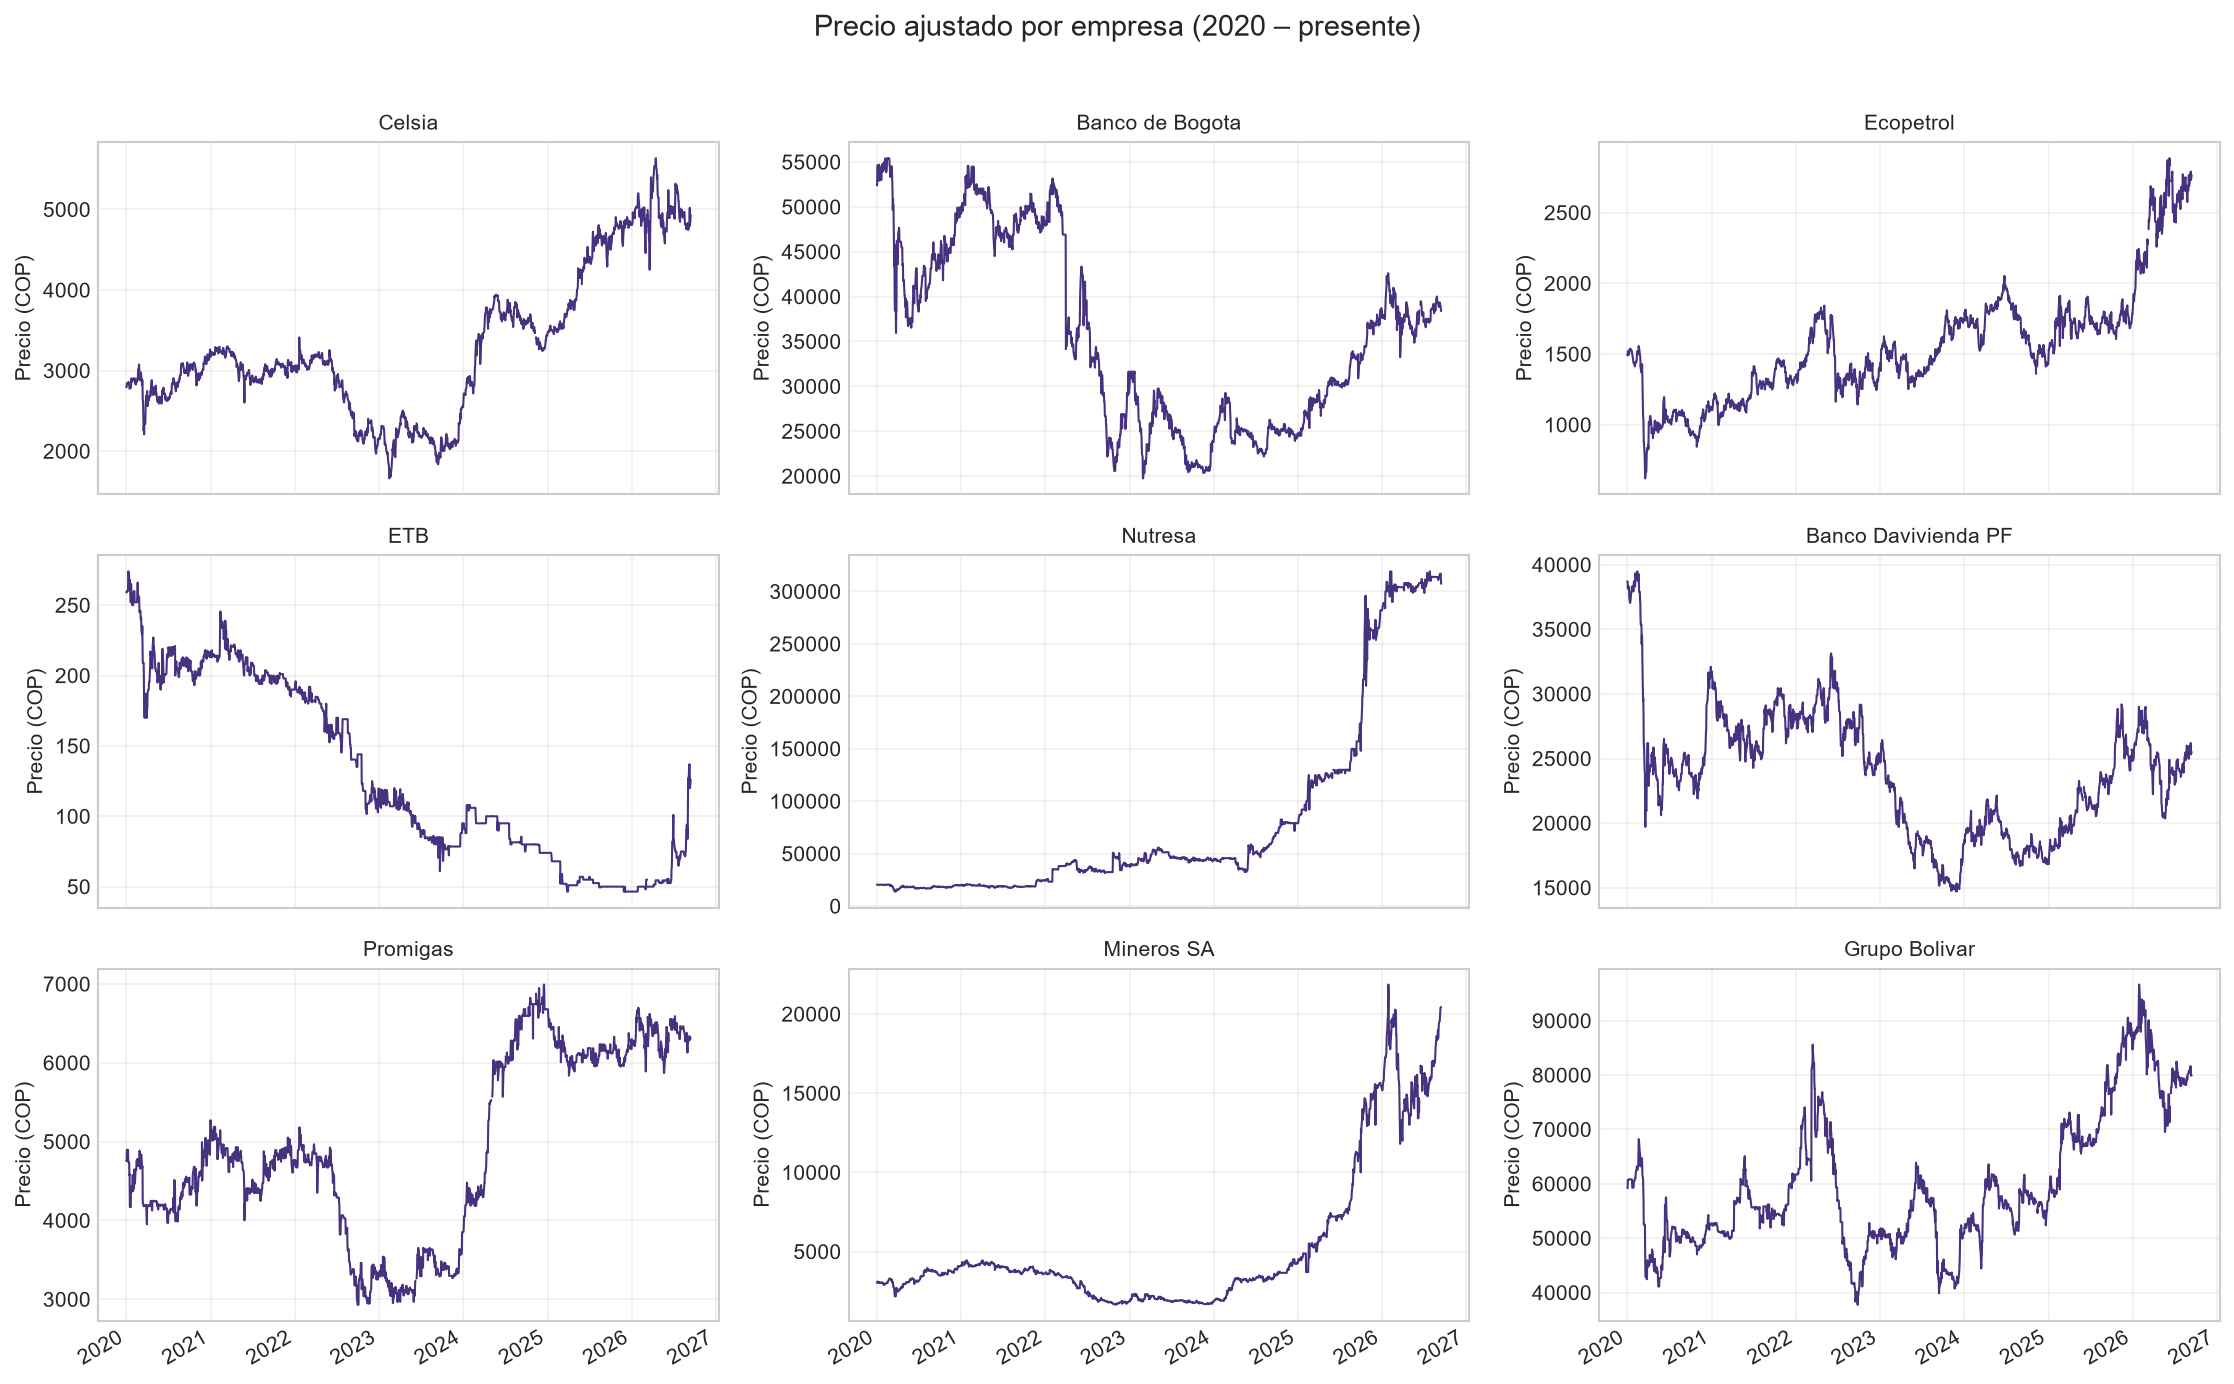
\includegraphics[width=\linewidth]{01_precios.png}
      \caption{Precio ajustado de las 9 acciones, en pesos colombianos.}
    \end{figure}

    \vspace{0.4cm}
    {\centering
    \begin{tikzpicture}[x=0.215cm,y=1cm]
      \fill[azulposter] (0,0) rectangle (36,1.8);
      \fill[azulposter!45] (36,0) rectangle (56,1.8);
      \fill[red!55!black] (56,0) rectangle (80,1.8);
      \node[white,font=\bfseries\small,align=center] at (18,0.9) {Entrenamiento\\2020--2023};
      \node[black,font=\bfseries\small,align=center] at (46,0.9) {Validación\\2024};
      \node[white,font=\bfseries\small,align=center] at (68,0.9) {Prueba\\2025--2026};
      \node[font=\small,below,align=center] at (18,-0.05) {estimar\\parámetros};
      \node[font=\small,below,align=center] at (46,-0.05) {elegir\\modelos};
      \node[font=\small,below,align=center] at (68,-0.05) {cerrada; se\\abrió \textbf{una vez}};
    \end{tikzpicture}\par}

    Las hipótesis de la evaluación final se registraron por escrito y se aprobaron \textbf{antes} de abrir el bloque de prueba (426 días).
  \end{block}

  \begin{alertblock}{Metodología}
    \begin{itemize}
      \item \textbf{Rendimiento logarítmico:} $r_t=\ln(P_t/P_{t-1})$; estacionario según ADF y KPSS (los precios no).
      \item \textbf{Econometría:} ARIMA elegido por BIC; GARCH(1,1) con errores $t$: $\sigma^2_t=\omega+\alpha\varepsilon^2_{t-1}+\beta\sigma^2_{t-1}$; HAR para la volatilidad semanal.
      \item \textbf{Referencia de volatilidad EWMA} (sin parámetros estimados): $\sigma^2_t=\lambda\sigma^2_{t-1}+(1-\lambda)r^2_{t-1}$, $\lambda=0{,}94$.
      \item \textbf{Aprendizaje automático:} Random Forest y Gradient Boosting con rezagos, volatilidades, volumen, TRM y Brent conocidos \textit{antes} del día pronosticado.
      \item \textbf{Redes neuronales:} MLP y LSTM (30 días de historia), parada temprana y promedio de 5 semillas.
      \item \textbf{Comparación:} Diebold-Mariano, Model Confidence Set y corrección de Holm; R$^2$ fuera de muestra frente a la media histórica.
      \item \textbf{Riesgo y portafolios:} VaR y ES al 99\,\% (normal-EWMA, histórica, FHS, GARCH-$t$) con Kupiec y Christoffersen; mínima varianza, Ledoit-Wolf, mínimo CVaR y paridad de riesgo frente al \textbf{1/N}, con máx.\ 30\,\% por acción, 40\,\% por sector, 20 pb de costos y Sharpe neto con el IBR.
    \end{itemize}
  \end{alertblock}

  \begin{block}{Agente de IA de investigación}
    Agente sobre Claude que consulta el diario de decisiones y los resultados, verifica la reproducibilidad y propone cambios para revisión humana, \textbf{sin poder modificar datos ni abrir la prueba}. Segunda evaluación (12 escenarios $\times$ 3 repeticiones, con trampas de fuga de información): \textbf{97,5\,\%} de criterios (193/198) y \textbf{100\,\%} de integridad.
  \end{block}

\end{column}

\separatorcolumn

\begin{column}{\colwidth}

  \begin{block}{Resultados en la prueba (2025--2026)}
    \textbf{1. Rendimiento diario: ningún modelo supera a la media histórica.}

    {\centering\small
    \begin{tabular}{lrr}
      \toprule
      Modelo & R$^2$ fuera de muestra [IC 95\,\%] & $p$ DM (Holm) \\
      \midrule
      LSTM & 1,79\,\% [$-$0,16; 3,86] & 0,58 \\
      Random Forest & 1,43\,\% [0,12; 2,83] & 0,58 \\
      Gradient Boosting & 1,37\,\% [$-$0,48; 3,43] & 0,70 \\
      MLP & 0,92\,\% [0,07; 1,83] & 0,40 \\
      ARIMA & $-$2,20\,\% & 0,70 \\
      \bottomrule
    \end{tabular}\par}

    Los siete modelos, incluida la media, quedan en el MCS.

    \textbf{2. Volatilidad: lo simple gana.} EWMA tiene la menor pérdida QLIKE (2,189); GARCH no la supera ($p=0{,}84$).

    \textbf{3. Riesgo: suponer normalidad subestima la cola.}

    {\centering\small
    \begin{tabular}{lrl}
      \toprule
      VaR 99\,\% (10 series) & Excesos & Lectura \\
      \midrule
      Esperados & 41 & \\
      Normal-EWMA & 55 & subestima la cola \\
      FHS & 29 & ES mejor calibrado \\
      GARCH-$t$ & 28 & conservador \\
      \bottomrule
    \end{tabular}\par}

    \textbf{4. Portafolios: ninguna estrategia supera al 1/N.} \$1 invertido en enero de 2025 terminó en \textbf{\$1,97 con 1/N} frente a \$1,74 con mínima varianza Ledoit-Wolf (Sharpe neto 1,98 frente a 1,59). El 1/N también ganó en las 24 configuraciones del análisis de robustez (2021--2026).

    \begin{figure}
      \centering
      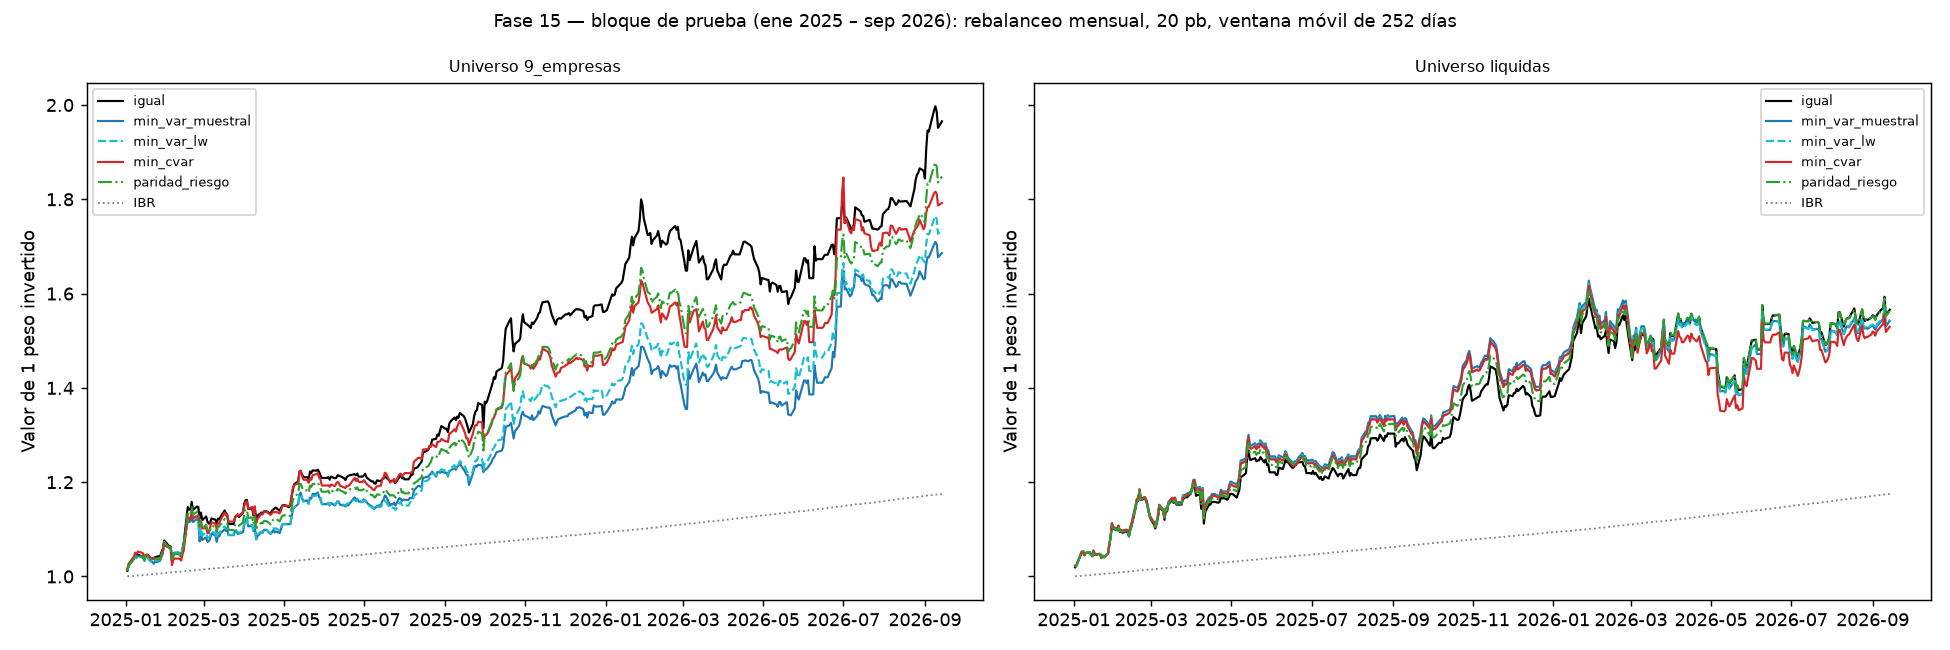
\includegraphics[width=\linewidth]{fase15_riqueza_prueba.png}
      \caption{Valor de \$1 invertido en la prueba, rebalanceo mensual y 20 pb de costos.}
    \end{figure}

    \begin{figure}
      \centering
      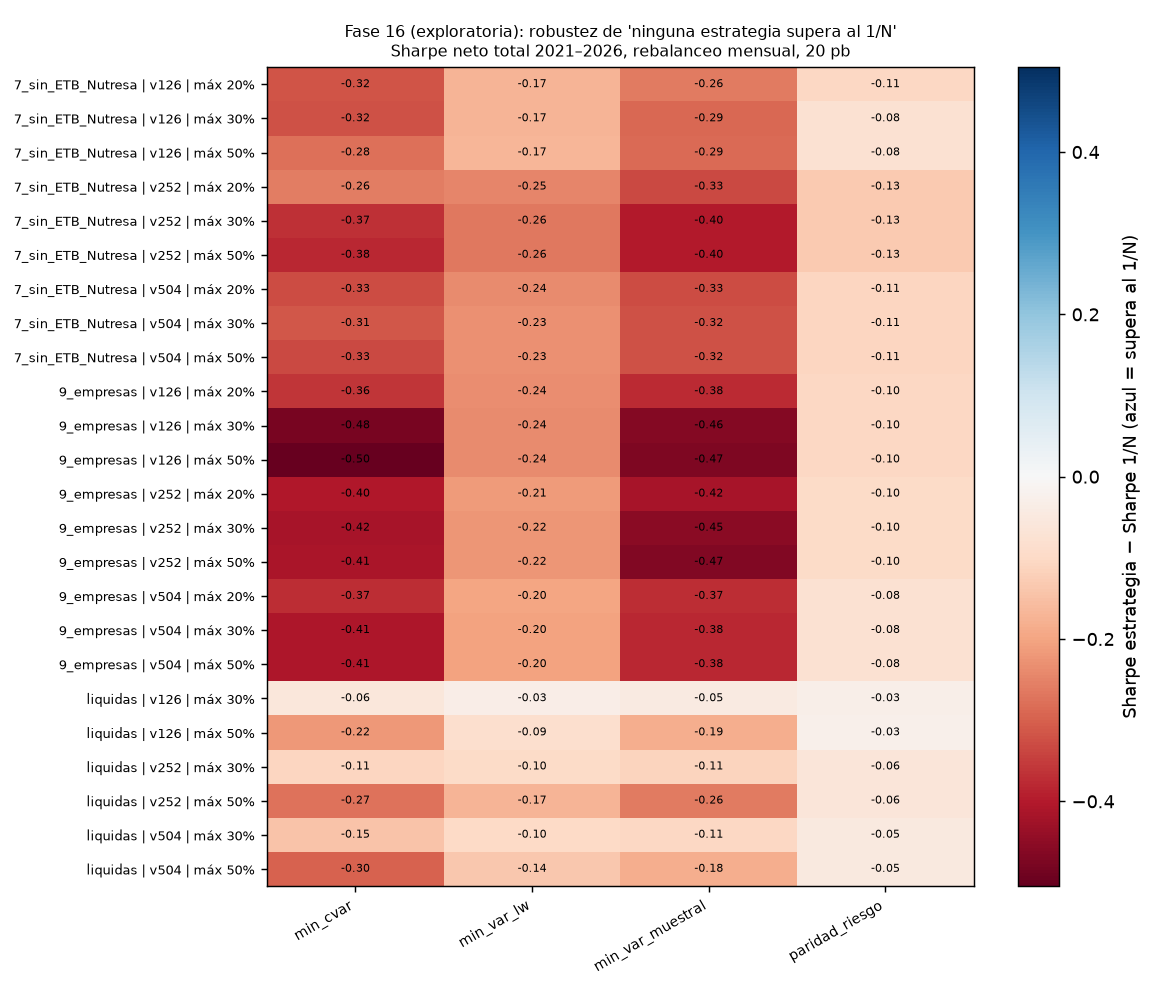
\includegraphics[width=0.6\linewidth]{fase16_robustez_portafolios.png}
      \caption{Robustez (exploratoria): diferencia de Sharpe neto frente al 1/N en 24 configuraciones; todas son negativas.}
    \end{figure}
  \end{block}

  \begin{block}{Conclusiones}
    \begin{itemize}
      \item Más complejidad no significó mejores pronósticos: la IA debe demostrar que mejora algo fuera de muestra.
      \item La volatilidad sí es predecible, y una referencia sin parámetros (EWMA) es difícil de superar.
      \item Para el riesgo extremo, suponer normalidad es peligroso; FHS está mejor calibrada.
      \item Predecir no es invertir bien: el portafolio 1/N no fue superado.
    \end{itemize}
    \textit{Con datos colombianos, ningún modelo complejo superó a referencias simples fuera de muestra; el protocolo preregistrado es lo que hace creíble este resultado.}
  \end{block}

  \begin{block}{Referencias}
    \footnotesize
    \begin{itemize}
      \item[{[1]}] V. DeMiguel, L. Garlappi y R. Uppal, ``Optimal versus naive diversification: How inefficient is the 1/N portfolio strategy?'', \textit{Rev. Financ. Stud.}, vol. 22, no. 5, pp. 1915--1953, 2009.
      \item[{[2]}] F. X. Diebold y R. S. Mariano, ``Comparing predictive accuracy'', \textit{J. Bus. Econ. Stat.}, vol. 13, no. 3, pp. 253--263, 1995.
      \item[{[3]}] P. R. Hansen, A. Lunde y J. M. Nason, ``The model confidence set'', \textit{Econometrica}, vol. 79, no. 2, pp. 453--497, 2011.
      \item[{[4]}] T. Bollerslev, ``Generalized autoregressive conditional heteroskedasticity'', \textit{J. Econometrics}, vol. 31, no. 3, pp. 307--327, 1986.
      \item[{[5]}] O. Ledoit y M. Wolf, ``A well-conditioned estimator for large-dimensional covariance matrices'', \textit{J. Multivariate Anal.}, vol. 88, no. 2, pp. 365--411, 2004.
    \end{itemize}
  \end{block}

\end{column}

\separatorcolumn
\end{columns}

% Logo institucional en la esquina inferior derecha
\begin{tikzpicture}[remember picture,overlay]
  \node[anchor=south east,inner sep=0pt]
    at ([xshift=-1.50cm,yshift=0.5cm]current page.south east)
    {
\includegraphics[width=2.8cm]{Logo.png}};
\end{tikzpicture}

\end{frame}

\end{document}
